% Options for packages loaded elsewhere
\PassOptionsToPackage{unicode}{hyperref}
\PassOptionsToPackage{hyphens}{url}
\PassOptionsToPackage{dvipsnames,svgnames,x11names}{xcolor}
%
\documentclass[
  11pt,
  a4paper,
]{scrartcl}
\title{Homework 3 Report}
\usepackage{etoolbox}
\makeatletter
\providecommand{\subtitle}[1]{% add subtitle to \maketitle
  \apptocmd{\@title}{\par {\large #1 \par}}{}{}
}
\makeatother
\subtitle{Classification of liver malfunction severity (LDA)}
\author{Ian Effendi \textbackslash{}
\href{mailto:iae2784@rit.edu}{\nolinkurl{iae2784@rit.edu}}}
\date{October 12, 2021}

\usepackage{amsmath,amssymb}
\usepackage{lmodern}
\usepackage{iftex}
\ifPDFTeX
  \usepackage[T1]{fontenc}
  \usepackage[utf8]{inputenc}
  \usepackage{textcomp} % provide euro and other symbols
\else % if luatex or xetex
  \usepackage{unicode-math}
  \defaultfontfeatures{Scale=MatchLowercase}
  \defaultfontfeatures[\rmfamily]{Ligatures=TeX,Scale=1}
\fi
% Use upquote if available, for straight quotes in verbatim environments
\IfFileExists{upquote.sty}{\usepackage{upquote}}{}
\IfFileExists{microtype.sty}{% use microtype if available
  \usepackage[]{microtype}
  \UseMicrotypeSet[protrusion]{basicmath} % disable protrusion for tt fonts
}{}
\makeatletter
\@ifundefined{KOMAClassName}{% if non-KOMA class
  \IfFileExists{parskip.sty}{%
    \usepackage{parskip}
  }{% else
    \setlength{\parindent}{0pt}
    \setlength{\parskip}{6pt plus 2pt minus 1pt}}
}{% if KOMA class
  \KOMAoptions{parskip=half}}
\makeatother
\usepackage{xcolor}
\IfFileExists{xurl.sty}{\usepackage{xurl}}{} % add URL line breaks if available
\IfFileExists{bookmark.sty}{\usepackage{bookmark}}{\usepackage{hyperref}}
\hypersetup{
  pdftitle={Homework 3 Report},
  pdfauthor={Ian Effendi \textbackslash{} iae2784@rit.edu},
  colorlinks=true,
  linkcolor={Maroon},
  filecolor={Maroon},
  citecolor={Blue},
  urlcolor={violet},
  pdfcreator={LaTeX via pandoc}}
\urlstyle{same} % disable monospaced font for URLs
\usepackage[margin=1in,heightrounded]{geometry}
\usepackage{color}
\usepackage{fancyvrb}
\newcommand{\VerbBar}{|}
\newcommand{\VERB}{\Verb[commandchars=\\\{\}]}
\DefineVerbatimEnvironment{Highlighting}{Verbatim}{commandchars=\\\{\}}
% Add ',fontsize=\small' for more characters per line
\usepackage{framed}
\definecolor{shadecolor}{RGB}{248,248,248}
\newenvironment{Shaded}{\begin{snugshade}}{\end{snugshade}}
\newcommand{\AlertTok}[1]{\textcolor[rgb]{0.94,0.16,0.16}{#1}}
\newcommand{\AnnotationTok}[1]{\textcolor[rgb]{0.56,0.35,0.01}{\textbf{\textit{#1}}}}
\newcommand{\AttributeTok}[1]{\textcolor[rgb]{0.77,0.63,0.00}{#1}}
\newcommand{\BaseNTok}[1]{\textcolor[rgb]{0.00,0.00,0.81}{#1}}
\newcommand{\BuiltInTok}[1]{#1}
\newcommand{\CharTok}[1]{\textcolor[rgb]{0.31,0.60,0.02}{#1}}
\newcommand{\CommentTok}[1]{\textcolor[rgb]{0.56,0.35,0.01}{\textit{#1}}}
\newcommand{\CommentVarTok}[1]{\textcolor[rgb]{0.56,0.35,0.01}{\textbf{\textit{#1}}}}
\newcommand{\ConstantTok}[1]{\textcolor[rgb]{0.00,0.00,0.00}{#1}}
\newcommand{\ControlFlowTok}[1]{\textcolor[rgb]{0.13,0.29,0.53}{\textbf{#1}}}
\newcommand{\DataTypeTok}[1]{\textcolor[rgb]{0.13,0.29,0.53}{#1}}
\newcommand{\DecValTok}[1]{\textcolor[rgb]{0.00,0.00,0.81}{#1}}
\newcommand{\DocumentationTok}[1]{\textcolor[rgb]{0.56,0.35,0.01}{\textbf{\textit{#1}}}}
\newcommand{\ErrorTok}[1]{\textcolor[rgb]{0.64,0.00,0.00}{\textbf{#1}}}
\newcommand{\ExtensionTok}[1]{#1}
\newcommand{\FloatTok}[1]{\textcolor[rgb]{0.00,0.00,0.81}{#1}}
\newcommand{\FunctionTok}[1]{\textcolor[rgb]{0.00,0.00,0.00}{#1}}
\newcommand{\ImportTok}[1]{#1}
\newcommand{\InformationTok}[1]{\textcolor[rgb]{0.56,0.35,0.01}{\textbf{\textit{#1}}}}
\newcommand{\KeywordTok}[1]{\textcolor[rgb]{0.13,0.29,0.53}{\textbf{#1}}}
\newcommand{\NormalTok}[1]{#1}
\newcommand{\OperatorTok}[1]{\textcolor[rgb]{0.81,0.36,0.00}{\textbf{#1}}}
\newcommand{\OtherTok}[1]{\textcolor[rgb]{0.56,0.35,0.01}{#1}}
\newcommand{\PreprocessorTok}[1]{\textcolor[rgb]{0.56,0.35,0.01}{\textit{#1}}}
\newcommand{\RegionMarkerTok}[1]{#1}
\newcommand{\SpecialCharTok}[1]{\textcolor[rgb]{0.00,0.00,0.00}{#1}}
\newcommand{\SpecialStringTok}[1]{\textcolor[rgb]{0.31,0.60,0.02}{#1}}
\newcommand{\StringTok}[1]{\textcolor[rgb]{0.31,0.60,0.02}{#1}}
\newcommand{\VariableTok}[1]{\textcolor[rgb]{0.00,0.00,0.00}{#1}}
\newcommand{\VerbatimStringTok}[1]{\textcolor[rgb]{0.31,0.60,0.02}{#1}}
\newcommand{\WarningTok}[1]{\textcolor[rgb]{0.56,0.35,0.01}{\textbf{\textit{#1}}}}
\usepackage{longtable,booktabs,array}
\usepackage{calc} % for calculating minipage widths
% Correct order of tables after \paragraph or \subparagraph
\usepackage{etoolbox}
\makeatletter
\patchcmd\longtable{\par}{\if@noskipsec\mbox{}\fi\par}{}{}
\makeatother
% Allow footnotes in longtable head/foot
\IfFileExists{footnotehyper.sty}{\usepackage{footnotehyper}}{\usepackage{footnote}}
\makesavenoteenv{longtable}
\usepackage{graphicx}
\makeatletter
\def\maxwidth{\ifdim\Gin@nat@width>\linewidth\linewidth\else\Gin@nat@width\fi}
\def\maxheight{\ifdim\Gin@nat@height>\textheight\textheight\else\Gin@nat@height\fi}
\makeatother
% Scale images if necessary, so that they will not overflow the page
% margins by default, and it is still possible to overwrite the defaults
% using explicit options in \includegraphics[width, height, ...]{}
\setkeys{Gin}{width=\maxwidth,height=\maxheight,keepaspectratio}
% Set default figure placement to htbp
\makeatletter
\def\fps@figure{htbp}
\makeatother
\setlength{\emergencystretch}{3em} % prevent overfull lines
\providecommand{\tightlist}{%
  \setlength{\itemsep}{0pt}\setlength{\parskip}{0pt}}
\setcounter{secnumdepth}{-\maxdimen} % remove section numbering
\ifLuaTeX
  \usepackage{selnolig}  % disable illegal ligatures
\fi

\begin{document}
\maketitle

{
\hypersetup{linkcolor=blue}
\setcounter{tocdepth}{3}
\tableofcontents
}
\hypertarget{certification}{%
\subsection{Certification}\label{certification}}

\begin{quote}
I certify that I indeed finished reading Ch. 4 from \emph{An
Introduction to Statistical Learning}, by James Gareth, Daniela Witten,
Trevor Hastie, Robert Tibshirani.
\end{quote}

\hypertarget{overview}{%
\subsection{Overview}\label{overview}}

In this assignment we will:

\begin{itemize}
\tightlist
\item
  Perform exploratory data analysis (\emph{EDA}) on the dataset.
\item
  Fit and analyze a linear discriminant analysis (\emph{LDA}) model on
  the dataset.
\item
  Perform multiple cross-validation tasks at different \(k\)-fold values
  (\(k=3,\,k=10\)).
\end{itemize}

\hypertarget{elt}{%
\subsection{ELT}\label{elt}}

\emph{Much of the \textbf{extract}, \textbf{load}, and
\textbf{transform} (\textbf{ELT}) process from the previous report has
been revised for this assignment. Notably, a \texttt{make.dataset()}
function streamlines the process of parsing the source
\texttt{Liver.txt} file into a compatible \texttt{data.frame}.}

\begin{Shaded}
\begin{Highlighting}[]
\CommentTok{\# Import the dataset as variable called "Liver".}
\FunctionTok{setup.analysis}\NormalTok{(}\AttributeTok{target =} \StringTok{"Liver"}\NormalTok{)}
\end{Highlighting}
\end{Shaded}

\begin{verbatim}
## Use cached dataset? TRUE
\end{verbatim}

\begin{verbatim}
## 'Liver' exists.
\end{verbatim}

\begin{verbatim}
## Importing dataset...
\end{verbatim}

\begin{verbatim}
## Parsing dataset from local file...
\end{verbatim}

\begin{verbatim}
## Reading dataset from compressed cache file...
\end{verbatim}

\begin{verbatim}
## Done.
\end{verbatim}

\begin{verbatim}
## Dataset imported.
\end{verbatim}

\begin{verbatim}
## Registered target dataset to global environment. Access using 'Liver'.
\end{verbatim}

\begin{verbatim}
## Use 'Liver' to access underlying tbl_df.
\end{verbatim}

\begin{verbatim}
## Dataset of type: 'tbl_df/tbl/data.frame'.
\end{verbatim}

\begin{longtable}[]{@{}rrrrrrl@{}}
\toprule
blood.1 & blood.2 & blood.3 & blood.4 & blood.5 & drinks & severity \\
\midrule
\endhead
85 & 92 & 45 & 27 & 31 & 0.0 & 1 \\
85 & 64 & 59 & 32 & 23 & 0.0 & 2 \\
86 & 54 & 33 & 16 & 54 & 0.0 & 2 \\
91 & 78 & 34 & 24 & 36 & 0.0 & 2 \\
87 & 70 & 12 & 28 & 10 & 0.0 & 2 \\
98 & 55 & 13 & 17 & 17 & 0.0 & 2 \\
88 & 62 & 20 & 17 & 9 & 0.5 & 1 \\
88 & 67 & 21 & 11 & 11 & 0.5 & 1 \\
92 & 54 & 22 & 20 & 7 & 0.5 & 1 \\
90 & 60 & 25 & 19 & 5 & 0.5 & 1 \\
89 & 52 & 13 & 24 & 15 & 0.5 & 1 \\
82 & 62 & 17 & 17 & 15 & 0.5 & 1 \\
90 & 64 & 61 & 32 & 13 & 0.5 & 1 \\
86 & 77 & 25 & 19 & 18 & 0.5 & 1 \\
96 & 67 & 29 & 20 & 11 & 0.5 & 1 \\
91 & 78 & 20 & 31 & 18 & 0.5 & 1 \\
89 & 67 & 23 & 16 & 10 & 0.5 & 1 \\
89 & 79 & 17 & 17 & 16 & 0.5 & 1 \\
91 & 107 & 20 & 20 & 56 & 0.5 & 1 \\
94 & 116 & 11 & 33 & 11 & 0.5 & 1 \\
92 & 59 & 35 & 13 & 19 & 0.5 & 1 \\
93 & 23 & 35 & 20 & 20 & 0.5 & 1 \\
90 & 60 & 23 & 27 & 5 & 0.5 & 1 \\
96 & 68 & 18 & 19 & 19 & 0.5 & 1 \\
84 & 80 & 47 & 33 & 97 & 0.5 & 1 \\
92 & 70 & 24 & 13 & 26 & 0.5 & 1 \\
90 & 47 & 28 & 15 & 18 & 0.5 & 1 \\
88 & 66 & 20 & 21 & 10 & 0.5 & 1 \\
91 & 102 & 17 & 13 & 19 & 0.5 & 1 \\
87 & 41 & 31 & 19 & 16 & 0.5 & 1 \\
86 & 79 & 28 & 16 & 17 & 0.5 & 1 \\
91 & 57 & 31 & 23 & 42 & 0.5 & 1 \\
93 & 77 & 32 & 18 & 29 & 0.5 & 1 \\
88 & 96 & 28 & 21 & 40 & 0.5 & 1 \\
94 & 65 & 22 & 18 & 11 & 0.5 & 1 \\
91 & 72 & 155 & 68 & 82 & 0.5 & 2 \\
85 & 54 & 47 & 33 & 22 & 0.5 & 2 \\
79 & 39 & 14 & 19 & 9 & 0.5 & 2 \\
85 & 85 & 25 & 26 & 30 & 0.5 & 2 \\
89 & 63 & 24 & 20 & 38 & 0.5 & 2 \\
84 & 92 & 68 & 37 & 44 & 0.5 & 2 \\
89 & 68 & 26 & 39 & 42 & 0.5 & 2 \\
89 & 101 & 18 & 25 & 13 & 0.5 & 2 \\
86 & 84 & 18 & 14 & 16 & 0.5 & 2 \\
85 & 65 & 25 & 14 & 18 & 0.5 & 2 \\
88 & 61 & 19 & 21 & 13 & 0.5 & 2 \\
92 & 56 & 14 & 16 & 10 & 0.5 & 2 \\
95 & 50 & 29 & 25 & 50 & 0.5 & 2 \\
91 & 75 & 24 & 22 & 11 & 0.5 & 2 \\
83 & 40 & 29 & 25 & 38 & 0.5 & 2 \\
89 & 74 & 19 & 23 & 16 & 0.5 & 2 \\
85 & 64 & 24 & 22 & 11 & 0.5 & 2 \\
92 & 57 & 64 & 36 & 90 & 0.5 & 2 \\
94 & 48 & 11 & 23 & 43 & 0.5 & 2 \\
87 & 52 & 21 & 19 & 30 & 0.5 & 2 \\
85 & 65 & 23 & 29 & 15 & 0.5 & 2 \\
84 & 82 & 21 & 21 & 19 & 0.5 & 2 \\
88 & 49 & 20 & 22 & 19 & 0.5 & 2 \\
96 & 67 & 26 & 26 & 36 & 0.5 & 2 \\
90 & 63 & 24 & 24 & 24 & 0.5 & 2 \\
90 & 45 & 33 & 34 & 27 & 0.5 & 2 \\
90 & 72 & 14 & 15 & 18 & 0.5 & 2 \\
91 & 55 & 4 & 8 & 13 & 0.5 & 2 \\
91 & 52 & 15 & 22 & 11 & 0.5 & 2 \\
87 & 71 & 32 & 19 & 27 & 1.0 & 1 \\
89 & 77 & 26 & 20 & 19 & 1.0 & 1 \\
89 & 67 & 5 & 17 & 14 & 1.0 & 2 \\
85 & 51 & 26 & 24 & 23 & 1.0 & 2 \\
103 & 75 & 19 & 30 & 13 & 1.0 & 2 \\
90 & 63 & 16 & 21 & 14 & 1.0 & 2 \\
90 & 63 & 29 & 23 & 57 & 2.0 & 1 \\
90 & 67 & 35 & 19 & 35 & 2.0 & 1 \\
87 & 66 & 27 & 22 & 9 & 2.0 & 1 \\
90 & 73 & 34 & 21 & 22 & 2.0 & 1 \\
86 & 54 & 20 & 21 & 16 & 2.0 & 1 \\
90 & 80 & 19 & 14 & 42 & 2.0 & 1 \\
87 & 90 & 43 & 28 & 156 & 2.0 & 2 \\
96 & 72 & 28 & 19 & 30 & 2.0 & 2 \\
91 & 55 & 9 & 25 & 16 & 2.0 & 2 \\
95 & 78 & 27 & 25 & 30 & 2.0 & 2 \\
92 & 101 & 34 & 30 & 64 & 2.0 & 2 \\
89 & 51 & 41 & 22 & 48 & 2.0 & 2 \\
91 & 99 & 42 & 33 & 16 & 2.0 & 2 \\
94 & 58 & 21 & 18 & 26 & 2.0 & 2 \\
92 & 60 & 30 & 27 & 297 & 2.0 & 2 \\
94 & 58 & 21 & 18 & 26 & 2.0 & 2 \\
88 & 47 & 33 & 26 & 29 & 2.0 & 2 \\
92 & 65 & 17 & 25 & 9 & 2.0 & 2 \\
92 & 79 & 22 & 20 & 11 & 3.0 & 1 \\
84 & 83 & 20 & 25 & 7 & 3.0 & 1 \\
88 & 68 & 27 & 21 & 26 & 3.0 & 1 \\
86 & 48 & 20 & 20 & 6 & 3.0 & 1 \\
99 & 69 & 45 & 32 & 30 & 3.0 & 1 \\
88 & 66 & 23 & 12 & 15 & 3.0 & 1 \\
89 & 62 & 42 & 30 & 20 & 3.0 & 1 \\
90 & 51 & 23 & 17 & 27 & 3.0 & 1 \\
81 & 61 & 32 & 37 & 53 & 3.0 & 2 \\
89 & 89 & 23 & 18 & 104 & 3.0 & 2 \\
89 & 65 & 26 & 18 & 36 & 3.0 & 2 \\
92 & 75 & 26 & 26 & 24 & 3.0 & 2 \\
85 & 59 & 25 & 20 & 25 & 3.0 & 2 \\
92 & 61 & 18 & 13 & 81 & 3.0 & 2 \\
89 & 63 & 22 & 27 & 10 & 4.0 & 1 \\
90 & 84 & 18 & 23 & 13 & 4.0 & 1 \\
88 & 95 & 25 & 19 & 14 & 4.0 & 1 \\
89 & 35 & 27 & 29 & 17 & 4.0 & 1 \\
91 & 80 & 37 & 23 & 27 & 4.0 & 1 \\
91 & 109 & 33 & 15 & 18 & 4.0 & 1 \\
91 & 65 & 17 & 5 & 7 & 4.0 & 1 \\
88 & 107 & 29 & 20 & 50 & 4.0 & 2 \\
87 & 76 & 22 & 55 & 9 & 4.0 & 2 \\
87 & 86 & 28 & 23 & 21 & 4.0 & 2 \\
87 & 42 & 26 & 23 & 17 & 4.0 & 2 \\
88 & 80 & 24 & 25 & 17 & 4.0 & 2 \\
90 & 96 & 34 & 49 & 169 & 4.0 & 2 \\
86 & 67 & 11 & 15 & 8 & 4.0 & 2 \\
92 & 40 & 19 & 20 & 21 & 4.0 & 2 \\
85 & 60 & 17 & 21 & 14 & 4.0 & 2 \\
89 & 90 & 15 & 17 & 25 & 4.0 & 2 \\
91 & 57 & 15 & 16 & 16 & 4.0 & 2 \\
96 & 55 & 48 & 39 & 42 & 4.0 & 2 \\
79 & 101 & 17 & 27 & 23 & 4.0 & 2 \\
90 & 134 & 14 & 20 & 14 & 4.0 & 2 \\
89 & 76 & 14 & 21 & 24 & 4.0 & 2 \\
88 & 93 & 29 & 27 & 31 & 4.0 & 2 \\
90 & 67 & 10 & 16 & 16 & 4.0 & 2 \\
92 & 73 & 24 & 21 & 48 & 4.0 & 2 \\
91 & 55 & 28 & 28 & 82 & 4.0 & 2 \\
83 & 45 & 19 & 21 & 13 & 4.0 & 2 \\
90 & 74 & 19 & 14 & 22 & 4.0 & 2 \\
92 & 66 & 21 & 16 & 33 & 5.0 & 1 \\
93 & 63 & 26 & 18 & 18 & 5.0 & 1 \\
86 & 78 & 47 & 39 & 107 & 5.0 & 2 \\
97 & 44 & 113 & 45 & 150 & 5.0 & 2 \\
87 & 59 & 15 & 19 & 12 & 5.0 & 2 \\
86 & 44 & 21 & 11 & 15 & 5.0 & 2 \\
87 & 64 & 16 & 20 & 24 & 5.0 & 2 \\
92 & 57 & 21 & 23 & 22 & 5.0 & 2 \\
90 & 70 & 25 & 23 & 112 & 5.0 & 2 \\
99 & 59 & 17 & 19 & 11 & 5.0 & 2 \\
92 & 80 & 10 & 26 & 20 & 6.0 & 1 \\
95 & 60 & 26 & 22 & 28 & 6.0 & 1 \\
91 & 63 & 25 & 26 & 15 & 6.0 & 1 \\
92 & 62 & 37 & 21 & 36 & 6.0 & 1 \\
95 & 50 & 13 & 14 & 15 & 6.0 & 1 \\
90 & 76 & 37 & 19 & 50 & 6.0 & 1 \\
96 & 70 & 70 & 26 & 36 & 6.0 & 1 \\
95 & 62 & 64 & 42 & 76 & 6.0 & 1 \\
92 & 62 & 20 & 23 & 20 & 6.0 & 1 \\
91 & 63 & 25 & 26 & 15 & 6.0 & 1 \\
82 & 56 & 67 & 38 & 92 & 6.0 & 2 \\
92 & 82 & 27 & 24 & 37 & 6.0 & 2 \\
90 & 63 & 12 & 26 & 21 & 6.0 & 2 \\
88 & 37 & 9 & 15 & 16 & 6.0 & 2 \\
100 & 60 & 29 & 23 & 76 & 6.0 & 2 \\
98 & 43 & 35 & 23 & 69 & 6.0 & 2 \\
91 & 74 & 87 & 50 & 67 & 6.0 & 2 \\
92 & 87 & 57 & 25 & 44 & 6.0 & 2 \\
93 & 99 & 36 & 34 & 48 & 6.0 & 2 \\
90 & 72 & 17 & 19 & 19 & 6.0 & 2 \\
97 & 93 & 21 & 20 & 68 & 6.0 & 2 \\
93 & 50 & 18 & 25 & 17 & 6.0 & 2 \\
90 & 57 & 20 & 26 & 33 & 6.0 & 2 \\
92 & 76 & 31 & 28 & 41 & 6.0 & 2 \\
88 & 55 & 19 & 17 & 14 & 6.0 & 2 \\
89 & 63 & 24 & 29 & 29 & 6.0 & 2 \\
92 & 79 & 70 & 32 & 84 & 7.0 & 1 \\
92 & 93 & 58 & 35 & 120 & 7.0 & 1 \\
93 & 84 & 58 & 47 & 62 & 7.0 & 2 \\
97 & 71 & 29 & 22 & 52 & 8.0 & 1 \\
84 & 99 & 33 & 19 & 26 & 8.0 & 1 \\
96 & 44 & 42 & 23 & 73 & 8.0 & 1 \\
90 & 62 & 22 & 21 & 21 & 8.0 & 1 \\
92 & 94 & 18 & 17 & 6 & 8.0 & 1 \\
90 & 67 & 77 & 39 & 114 & 8.0 & 1 \\
97 & 71 & 29 & 22 & 52 & 8.0 & 1 \\
91 & 69 & 25 & 25 & 66 & 8.0 & 2 \\
93 & 59 & 17 & 20 & 14 & 8.0 & 2 \\
92 & 95 & 85 & 48 & 200 & 8.0 & 2 \\
90 & 50 & 26 & 22 & 53 & 8.0 & 2 \\
91 & 62 & 59 & 47 & 60 & 8.0 & 2 \\
92 & 93 & 22 & 28 & 123 & 9.0 & 1 \\
92 & 77 & 86 & 41 & 31 & 10.0 & 1 \\
86 & 66 & 22 & 24 & 26 & 10.0 & 2 \\
98 & 57 & 31 & 34 & 73 & 10.0 & 2 \\
95 & 80 & 50 & 64 & 55 & 10.0 & 2 \\
92 & 108 & 53 & 33 & 94 & 12.0 & 2 \\
97 & 92 & 22 & 28 & 49 & 12.0 & 2 \\
93 & 77 & 39 & 37 & 108 & 16.0 & 1 \\
94 & 83 & 81 & 34 & 201 & 20.0 & 1 \\
87 & 75 & 25 & 21 & 14 & 0.0 & 1 \\
88 & 56 & 23 & 18 & 12 & 0.0 & 1 \\
84 & 97 & 41 & 20 & 32 & 0.0 & 2 \\
94 & 91 & 27 & 20 & 15 & 0.5 & 1 \\
97 & 62 & 17 & 13 & 5 & 0.5 & 1 \\
92 & 85 & 25 & 20 & 12 & 0.5 & 1 \\
82 & 48 & 27 & 15 & 12 & 0.5 & 1 \\
88 & 74 & 31 & 25 & 15 & 0.5 & 1 \\
95 & 77 & 30 & 14 & 21 & 0.5 & 1 \\
88 & 94 & 26 & 18 & 8 & 0.5 & 1 \\
91 & 70 & 19 & 19 & 22 & 0.5 & 1 \\
83 & 54 & 27 & 15 & 12 & 0.5 & 1 \\
91 & 105 & 40 & 26 & 56 & 0.5 & 1 \\
86 & 79 & 37 & 28 & 14 & 0.5 & 1 \\
91 & 96 & 35 & 22 & 135 & 0.5 & 1 \\
89 & 82 & 23 & 14 & 35 & 0.5 & 1 \\
90 & 73 & 24 & 23 & 11 & 0.5 & 1 \\
90 & 87 & 19 & 25 & 19 & 0.5 & 1 \\
89 & 82 & 33 & 32 & 18 & 0.5 & 1 \\
85 & 79 & 17 & 8 & 9 & 0.5 & 1 \\
85 & 119 & 30 & 26 & 17 & 0.5 & 1 \\
78 & 69 & 24 & 18 & 31 & 0.5 & 1 \\
88 & 107 & 34 & 21 & 27 & 0.5 & 1 \\
89 & 115 & 17 & 27 & 7 & 0.5 & 1 \\
92 & 67 & 23 & 15 & 12 & 0.5 & 1 \\
89 & 101 & 27 & 34 & 14 & 0.5 & 1 \\
91 & 84 & 11 & 12 & 10 & 0.5 & 1 \\
94 & 101 & 41 & 20 & 53 & 0.5 & 2 \\
88 & 46 & 29 & 22 & 18 & 0.5 & 2 \\
88 & 122 & 35 & 29 & 42 & 0.5 & 2 \\
84 & 88 & 28 & 25 & 35 & 0.5 & 2 \\
90 & 79 & 18 & 15 & 24 & 0.5 & 2 \\
87 & 69 & 22 & 26 & 11 & 0.5 & 2 \\
65 & 63 & 19 & 20 & 14 & 0.5 & 2 \\
90 & 64 & 12 & 17 & 14 & 0.5 & 2 \\
85 & 58 & 18 & 24 & 16 & 0.5 & 2 \\
88 & 81 & 41 & 27 & 36 & 0.5 & 2 \\
86 & 78 & 52 & 29 & 62 & 0.5 & 2 \\
82 & 74 & 38 & 28 & 48 & 0.5 & 2 \\
86 & 58 & 36 & 27 & 59 & 0.5 & 2 \\
94 & 56 & 30 & 18 & 27 & 0.5 & 2 \\
87 & 57 & 30 & 30 & 22 & 0.5 & 2 \\
98 & 74 & 148 & 75 & 159 & 0.5 & 2 \\
94 & 75 & 20 & 25 & 38 & 0.5 & 2 \\
83 & 68 & 17 & 20 & 71 & 0.5 & 2 \\
93 & 56 & 25 & 21 & 33 & 0.5 & 2 \\
101 & 65 & 18 & 21 & 22 & 0.5 & 2 \\
92 & 65 & 25 & 20 & 31 & 0.5 & 2 \\
92 & 58 & 14 & 16 & 13 & 0.5 & 2 \\
86 & 58 & 16 & 23 & 23 & 0.5 & 2 \\
85 & 62 & 15 & 13 & 22 & 0.5 & 2 \\
86 & 57 & 13 & 20 & 13 & 0.5 & 2 \\
86 & 54 & 26 & 30 & 13 & 0.5 & 2 \\
81 & 41 & 33 & 27 & 34 & 1.0 & 1 \\
91 & 67 & 32 & 26 & 13 & 1.0 & 1 \\
91 & 80 & 21 & 19 & 14 & 1.0 & 1 \\
92 & 60 & 23 & 15 & 19 & 1.0 & 1 \\
91 & 60 & 32 & 14 & 8 & 1.0 & 1 \\
93 & 65 & 28 & 22 & 10 & 1.0 & 1 \\
90 & 63 & 45 & 24 & 85 & 1.0 & 2 \\
87 & 92 & 21 & 22 & 37 & 1.0 & 2 \\
83 & 78 & 31 & 19 & 115 & 1.0 & 2 \\
95 & 62 & 24 & 23 & 14 & 1.0 & 2 \\
93 & 59 & 41 & 30 & 48 & 1.0 & 2 \\
84 & 82 & 43 & 32 & 38 & 2.0 & 1 \\
87 & 71 & 33 & 20 & 22 & 2.0 & 1 \\
86 & 44 & 24 & 15 & 18 & 2.0 & 1 \\
86 & 66 & 28 & 24 & 21 & 2.0 & 1 \\
88 & 58 & 31 & 17 & 17 & 2.0 & 1 \\
90 & 61 & 28 & 29 & 31 & 2.0 & 1 \\
88 & 69 & 70 & 24 & 64 & 2.0 & 1 \\
93 & 87 & 18 & 17 & 26 & 2.0 & 1 \\
98 & 58 & 33 & 21 & 28 & 2.0 & 1 \\
91 & 44 & 18 & 18 & 23 & 2.0 & 2 \\
87 & 75 & 37 & 19 & 70 & 2.0 & 2 \\
94 & 91 & 30 & 26 & 25 & 2.0 & 2 \\
88 & 85 & 14 & 15 & 10 & 2.0 & 2 \\
89 & 109 & 26 & 25 & 27 & 2.0 & 2 \\
87 & 59 & 37 & 27 & 34 & 2.0 & 2 \\
93 & 58 & 20 & 23 & 18 & 2.0 & 2 \\
88 & 57 & 9 & 15 & 16 & 2.0 & 2 \\
94 & 65 & 38 & 27 & 17 & 3.0 & 1 \\
91 & 71 & 12 & 22 & 11 & 3.0 & 1 \\
90 & 55 & 20 & 20 & 16 & 3.0 & 1 \\
91 & 64 & 21 & 17 & 26 & 3.0 & 2 \\
88 & 47 & 35 & 26 & 33 & 3.0 & 2 \\
82 & 72 & 31 & 20 & 84 & 3.0 & 2 \\
85 & 58 & 83 & 49 & 51 & 3.0 & 2 \\
91 & 54 & 25 & 22 & 35 & 4.0 & 1 \\
98 & 50 & 27 & 25 & 53 & 4.0 & 2 \\
86 & 62 & 29 & 21 & 26 & 4.0 & 2 \\
89 & 48 & 32 & 22 & 14 & 4.0 & 2 \\
82 & 68 & 20 & 22 & 9 & 4.0 & 2 \\
83 & 70 & 17 & 19 & 23 & 4.0 & 2 \\
96 & 70 & 21 & 26 & 21 & 4.0 & 2 \\
94 & 117 & 77 & 56 & 52 & 4.0 & 2 \\
93 & 45 & 11 & 14 & 21 & 4.0 & 2 \\
93 & 49 & 27 & 21 & 29 & 4.0 & 2 \\
84 & 73 & 46 & 32 & 39 & 4.0 & 2 \\
91 & 63 & 17 & 17 & 46 & 4.0 & 2 \\
90 & 57 & 31 & 18 & 37 & 4.0 & 2 \\
87 & 45 & 19 & 13 & 16 & 4.0 & 2 \\
91 & 68 & 14 & 20 & 19 & 4.0 & 2 \\
86 & 55 & 29 & 35 & 108 & 4.0 & 2 \\
91 & 86 & 52 & 47 & 52 & 4.0 & 2 \\
88 & 46 & 15 & 33 & 55 & 4.0 & 2 \\
85 & 52 & 22 & 23 & 34 & 4.0 & 2 \\
89 & 72 & 33 & 27 & 55 & 4.0 & 2 \\
95 & 59 & 23 & 18 & 19 & 4.0 & 2 \\
94 & 43 & 154 & 82 & 121 & 4.0 & 2 \\
96 & 56 & 38 & 26 & 23 & 5.0 & 2 \\
90 & 52 & 10 & 17 & 12 & 5.0 & 2 \\
94 & 45 & 20 & 16 & 12 & 5.0 & 2 \\
99 & 42 & 14 & 21 & 49 & 5.0 & 2 \\
93 & 102 & 47 & 23 & 37 & 5.0 & 2 \\
94 & 71 & 25 & 26 & 31 & 5.0 & 2 \\
92 & 73 & 33 & 34 & 115 & 5.0 & 2 \\
87 & 54 & 41 & 29 & 23 & 6.0 & 1 \\
92 & 67 & 15 & 14 & 14 & 6.0 & 1 \\
98 & 101 & 31 & 26 & 32 & 6.0 & 1 \\
92 & 53 & 51 & 33 & 92 & 6.0 & 1 \\
97 & 94 & 43 & 43 & 82 & 6.0 & 1 \\
93 & 43 & 11 & 16 & 54 & 6.0 & 1 \\
93 & 68 & 24 & 18 & 19 & 6.0 & 1 \\
95 & 36 & 38 & 19 & 15 & 6.0 & 1 \\
99 & 86 & 58 & 42 & 203 & 6.0 & 1 \\
98 & 66 & 103 & 57 & 114 & 6.0 & 1 \\
92 & 80 & 10 & 26 & 20 & 6.0 & 1 \\
96 & 74 & 27 & 25 & 43 & 6.0 & 2 \\
95 & 93 & 21 & 27 & 47 & 6.0 & 2 \\
86 & 109 & 16 & 22 & 28 & 6.0 & 2 \\
91 & 46 & 30 & 24 & 39 & 7.0 & 2 \\
102 & 82 & 34 & 78 & 203 & 7.0 & 2 \\
85 & 50 & 12 & 18 & 14 & 7.0 & 2 \\
91 & 57 & 33 & 23 & 12 & 8.0 & 1 \\
91 & 52 & 76 & 32 & 24 & 8.0 & 1 \\
93 & 70 & 46 & 30 & 33 & 8.0 & 1 \\
87 & 55 & 36 & 19 & 25 & 8.0 & 1 \\
98 & 123 & 28 & 24 & 31 & 8.0 & 1 \\
82 & 55 & 18 & 23 & 44 & 8.0 & 2 \\
95 & 73 & 20 & 25 & 225 & 8.0 & 2 \\
97 & 80 & 17 & 20 & 53 & 8.0 & 2 \\
100 & 83 & 25 & 24 & 28 & 8.0 & 2 \\
88 & 91 & 56 & 35 & 126 & 9.0 & 2 \\
91 & 138 & 45 & 21 & 48 & 10.0 & 1 \\
92 & 41 & 37 & 22 & 37 & 10.0 & 1 \\
86 & 123 & 20 & 25 & 23 & 10.0 & 2 \\
91 & 93 & 35 & 34 & 37 & 10.0 & 2 \\
87 & 87 & 15 & 23 & 11 & 10.0 & 2 \\
87 & 56 & 52 & 43 & 55 & 10.0 & 2 \\
99 & 75 & 26 & 24 & 41 & 12.0 & 1 \\
96 & 69 & 53 & 43 & 203 & 12.0 & 2 \\
98 & 77 & 55 & 35 & 89 & 15.0 & 1 \\
91 & 68 & 27 & 26 & 14 & 16.0 & 1 \\
98 & 99 & 57 & 45 & 65 & 20.0 & 1 \\
\bottomrule
\end{longtable}

The \texttt{setup.analysis()} function imports a dataset into the global
environment with the name provided to the \texttt{target\ =} argument.

\hypertarget{eda}{%
\subsection{EDA}\label{eda}}

\emph{This section reviews the \texttt{Liver} dataset. In an improvement
over the previous report, it now incorporates an assessment of feature
correlations.}

\hypertarget{response-encoding}{%
\subsubsection{Response Encoding}\label{response-encoding}}

\begin{Shaded}
\begin{Highlighting}[]
\CommentTok{\# Recode the response.}
\NormalTok{liver }\OtherTok{\textless{}{-}}\NormalTok{ Liver }\SpecialCharTok{\%\textgreater{}\%} \FunctionTok{make.response}\NormalTok{()}
\FunctionTok{summary}\NormalTok{(liver)}
\end{Highlighting}
\end{Shaded}

\begin{verbatim}
##     blood.1         blood.2         blood.3     
##  Min.   : 65.0   Min.   : 23.0   Min.   :  4.0  
##  1st Qu.: 87.0   1st Qu.: 57.0   1st Qu.: 19.0  
##  Median : 90.0   Median : 67.0   Median : 26.0  
##  Mean   : 90.2   Mean   : 69.9   Mean   : 30.4  
##  3rd Qu.: 93.0   3rd Qu.: 80.0   3rd Qu.: 34.0  
##  Max.   :103.0   Max.   :138.0   Max.   :155.0  
##     blood.4        blood.5          drinks     
##  Min.   : 5.0   Min.   :  5.0   Min.   : 0.00  
##  1st Qu.:19.0   1st Qu.: 15.0   1st Qu.: 0.50  
##  Median :23.0   Median : 25.0   Median : 3.00  
##  Mean   :24.6   Mean   : 38.3   Mean   : 3.46  
##  3rd Qu.:27.0   3rd Qu.: 46.0   3rd Qu.: 6.00  
##  Max.   :82.0   Max.   :297.0   Max.   :20.00  
##        severity  
##  Not Severe:200  
##  Severe    :145  
##                  
##                  
##                  
## 
\end{verbatim}

\begin{Shaded}
\begin{Highlighting}[]
\NormalTok{truth }\OtherTok{\textless{}{-}}\NormalTok{ (liver}\SpecialCharTok{$}\NormalTok{severity }\SpecialCharTok{==} \StringTok{"Severe"}\NormalTok{)}
\end{Highlighting}
\end{Shaded}

\newpage

\hypertarget{feature-correlations}{%
\subsubsection{Feature Correlations}\label{feature-correlations}}

\begin{Shaded}
\begin{Highlighting}[]
\NormalTok{liver.info }\OtherTok{\textless{}{-}} \FunctionTok{analysis.eda}\NormalTok{(Liver, truth)}
\FunctionTok{summary}\NormalTok{(liver.info)}
\end{Highlighting}
\end{Shaded}

\begin{verbatim}
##  n_samples n_features 
##        345          7 
## Label counts: 
##   pos   neg total 
##   145   200   345 
## Class prior probabilities: 
##    pos    neg 
## 0.4203 0.5797
\end{verbatim}

\begin{Shaded}
\begin{Highlighting}[]
\CommentTok{\# Plot using corrplot::corrplot wrapper.}
\NormalTok{liver.corrplot }\OtherTok{\textless{}{-}} \FunctionTok{corr.plot}\NormalTok{(}
\NormalTok{  liver, }\AttributeTok{sig.level =} \FloatTok{0.05}\NormalTok{, }\AttributeTok{insig =} \StringTok{"blank"}\NormalTok{,}
  \AttributeTok{title =} \StringTok{"Correlation Plot"}\NormalTok{,}
  \AttributeTok{mar =} \FunctionTok{c}\NormalTok{(}\DecValTok{1}\NormalTok{,}\DecValTok{1}\NormalTok{,}\DecValTok{2}\NormalTok{,}\DecValTok{1}\NormalTok{)}
\NormalTok{)}
\end{Highlighting}
\end{Shaded}

\begin{center}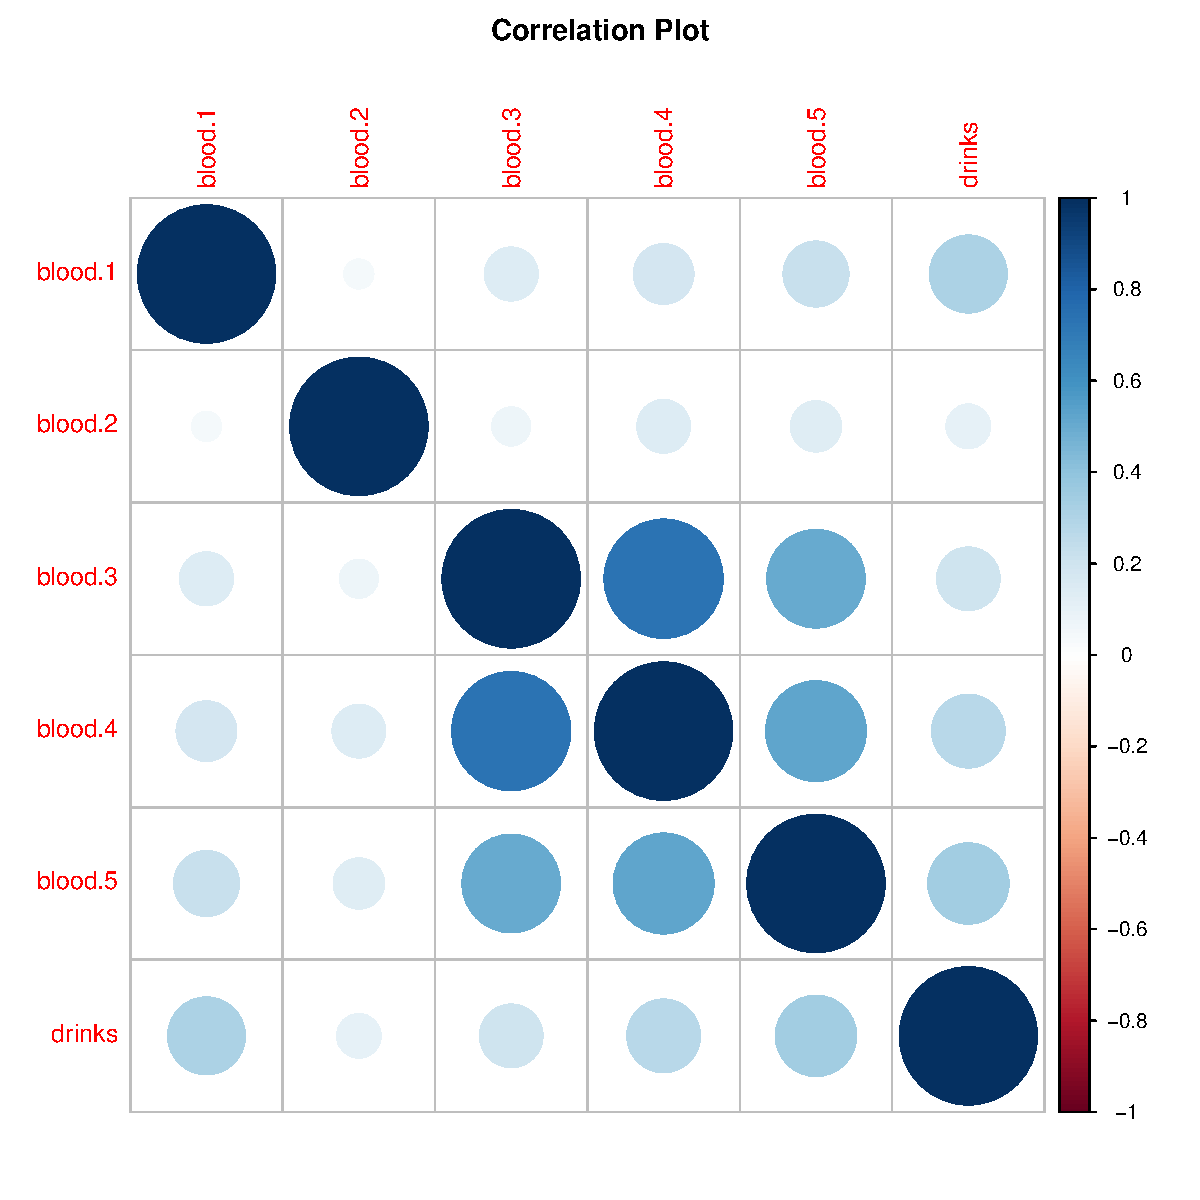
\includegraphics{figure/analysis-eda-corrplot-1} \end{center}

The data behind the above correlation plot is provided below:

\begin{verbatim}
## Feature correlation matrix: 
##         blood.1 blood.2 blood.3 blood.4 blood.5 drinks
## blood.1  1.0000 0.04410 0.14770  0.1878  0.2223 0.3127
## blood.2  0.0441 1.00000 0.07621  0.1461  0.1331 0.1008
## blood.3  0.1477 0.07621 1.00000  0.7397  0.5034 0.2068
## blood.4  0.1878 0.14606 0.73967  1.0000  0.5276 0.2796
## blood.5  0.2223 0.13314 0.50344  0.5276  1.0000 0.3412
## drinks   0.3127 0.10080 0.20685  0.2796  0.3412 1.0000
\end{verbatim}

\hypertarget{baseline-model-analysis}{%
\subsubsection{Baseline Model Analysis}\label{baseline-model-analysis}}

\begin{Shaded}
\begin{Highlighting}[]
\CommentTok{\# }\AlertTok{TODO}\CommentTok{: Replace glm with lda model.}
\NormalTok{liver.baseline }\OtherTok{\textless{}{-}} \FunctionTok{analysis.clf}\NormalTok{(}
\NormalTok{  liver, truth,}
  \AttributeTok{algorithm =}\NormalTok{ glm,}
  \AttributeTok{params =} \FunctionTok{list}\NormalTok{(}
    \AttributeTok{formula =}\NormalTok{ severity }\SpecialCharTok{\textasciitilde{}}\NormalTok{ .,}
    \AttributeTok{family =} \StringTok{"binomial"}
\NormalTok{  ),}
  \AttributeTok{pos =} \StringTok{"Severe"}\NormalTok{, }\AttributeTok{neg =} \StringTok{"Not Severe"}
\NormalTok{)}
\end{Highlighting}
\end{Shaded}

\begin{verbatim}
## Summary of baseline model: 
## 
## Call:
## "glm(formula = severity ~ ., family = binomial, data = liver)"
## 
## Deviance Residuals: 
##    Min      1Q  Median      3Q     Max  
## -1.964  -0.965  -0.591   1.048   2.419  
## 
## Coefficients:
##             Estimate Std. Error z value Pr(>|z|)    
## (Intercept) -5.99026    2.68546   -2.23  0.02571 *  
## blood.1      0.06398    0.02964    2.16  0.03090 *  
## blood.2      0.01953    0.00676    2.89  0.00387 ** 
## blood.3      0.06411    0.01230    5.21  1.9e-07 ***
## blood.4     -0.12320    0.02427   -5.08  3.9e-07 ***
## blood.5     -0.01895    0.00560   -3.38  0.00072 ***
## drinks       0.06808    0.04038    1.69  0.09179 .  
## ---
## Signif. codes:  
## 0 '***' 0.001 '**' 0.01 '*' 0.05 '.' 0.1 ' ' 1
## 
## (Dispersion parameter for binomial family taken to be 1)
## 
##     Null deviance: 469.47  on 344  degrees of freedom
## Residual deviance: 411.01  on 338  degrees of freedom
## AIC: 425
## 
## Number of Fisher Scoring iterations: 5
\end{verbatim}

\begin{verbatim}
## Baseline classification table: 
## Baseline model error rate: 
##                     0.3304 
##             truth
## predictions  Not Severe Severe
##   Not Severe        129     43
##   Severe             71    102
\end{verbatim}

\begin{center}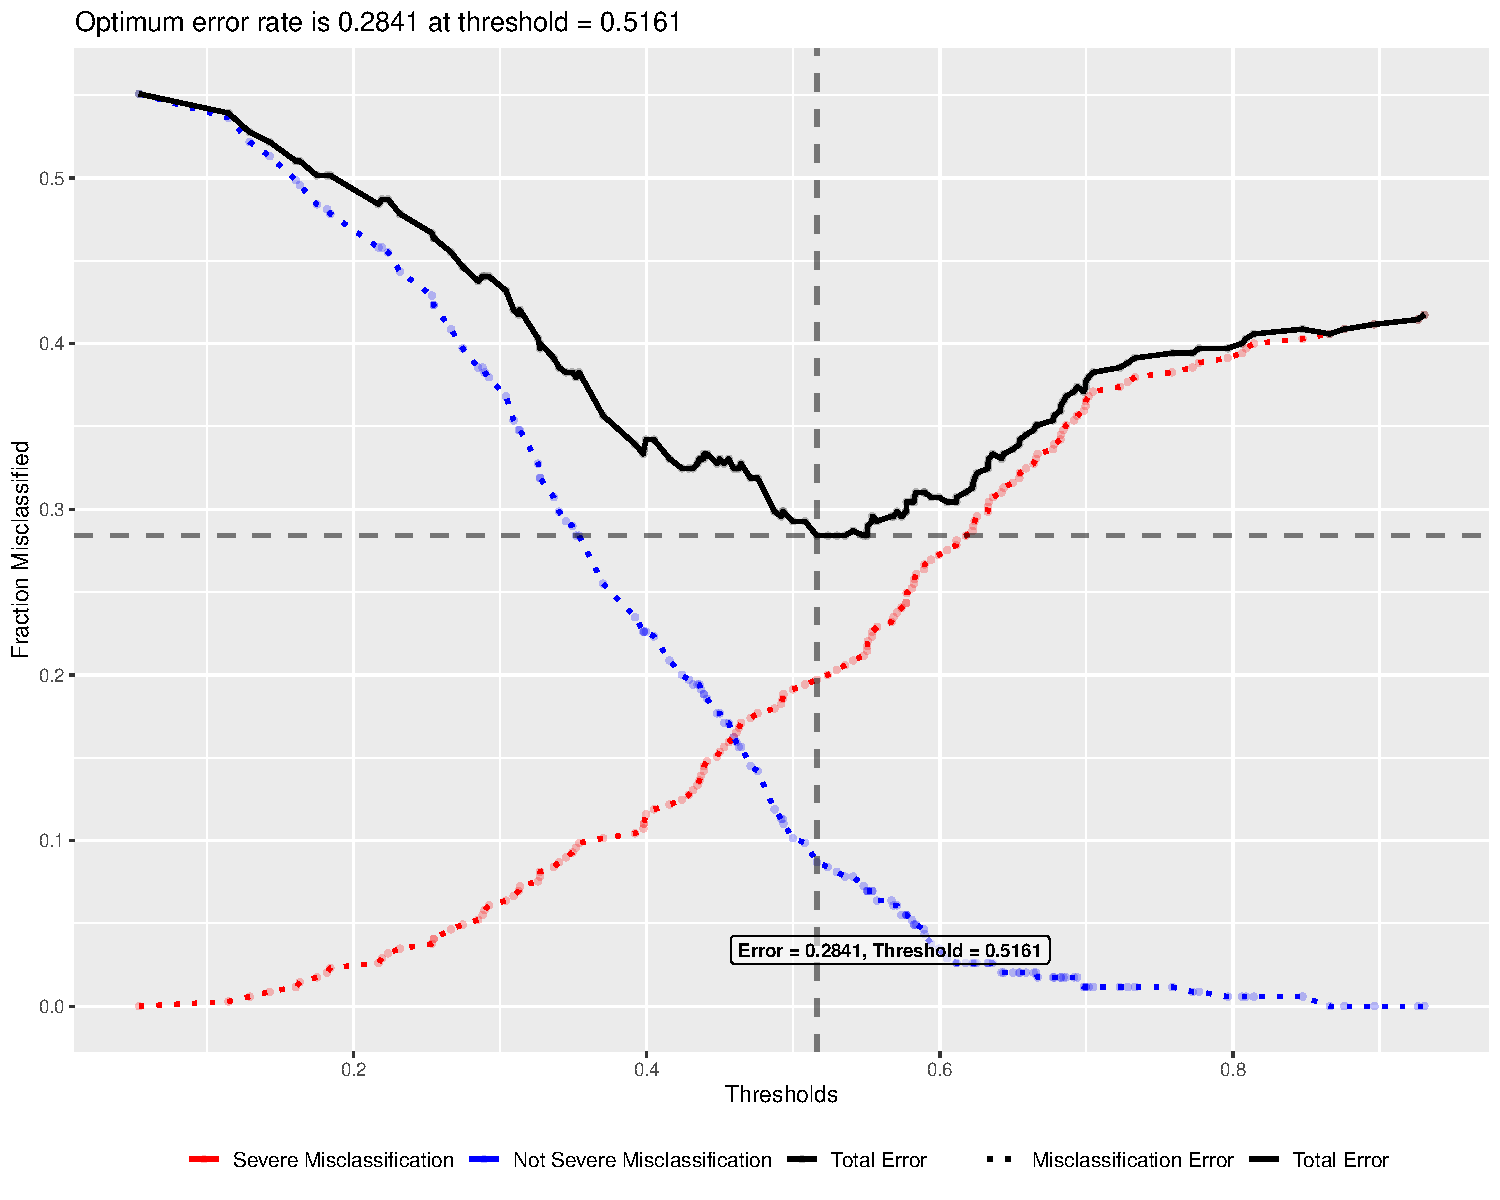
\includegraphics{figure/analysis-glm-optimal-error-1} \end{center}

\begin{verbatim}
## Misclassification table using optimal threshold: 
## Number of cases in table: 345 
## Number of factors: 2 
## Test for independence of all factors:
##  Chisq = 57, df = 1, p-value = 4e-14
##                    truth
## optimal_predictions Not Severe Severe
##          Not Severe        170     68
##          Severe             30     77
\end{verbatim}

\newpage

\hypertarget{cross-validation-analysis}{%
\subsection{Cross-Validation Analysis}\label{cross-validation-analysis}}

\hypertarget{fold-cv}{%
\subsubsection{10-fold CV}\label{fold-cv}}

\begin{verbatim}
## ---------------------------
## Performing 10-fold CV:
## # Samples: 345
## # Thresholds: 100
## # k folds: 10 || # rounds: 100
## ---------------------------
## tibble [100 x 4] (S3: tbl_df/tbl/data.frame)
##  $ total.err : num [1:100] 0.58 0.57 0.566 0.562 0.558 ...
##  $ ci.low    : num [1:100] 0.575 0.565 0.561 0.557 0.552 ...
##  $ ci.high   : num [1:100] 0.585 0.575 0.572 0.567 0.563 ...
##  $ thresholds: num [1:100] 0 0.0101 0.0202 0.0303 0.0404 ...
## tibble [300 x 4] (S3: tbl_df/tbl/data.frame)
##  $ thresholds: num [1:300] 0 0 0 0.0101 0.0101 ...
##  $ category  : chr [1:300] "total.err" "ci.low" "ci.high" "total.err" ...
##  $ error     : num [1:300] 0.58 0.575 0.585 0.57 0.565 ...
##  $ linetype  : logi [1:300] TRUE FALSE FALSE TRUE FALSE FALSE ...
## ---------------------------
## Calculating 10-fold CV table:
## # Samples: 345
## # Threshold: 1
## # k folds: 10 || # rounds: 100
## ---------------------------
##                       Length Class  Mode   
## results                  2   -none- list   
## plot                     2   -none- list   
## optimal_threshold        1   -none- numeric
## confusion_mat         4000   -none- numeric
## confusion_mat_summary    2   -none- list
\end{verbatim}

\begin{center}\includegraphics{figure/analysis-glm-10cv-plot-1} \end{center}

\begin{verbatim}
## $plot
## 
## $optimal_threshold
## [1] 0.5253
\end{verbatim}

\begin{verbatim}
## Optimal threshold: 0.525252525252525
## $mean
##        [,1]  [,2]
## [1,] 167.79 73.12
## [2,]  32.21 71.88
## 
## $sterr
##        [,1]   [,2]
## [1,] 0.2061 0.1876
## [2,] 0.2061 0.1876
\end{verbatim}

\newpage

\hypertarget{fold-cv-1}{%
\subsubsection{3-fold CV}\label{fold-cv-1}}

\begin{verbatim}
## ---------------------------
## Performing 3-fold CV:
## # Samples: 345
## # Thresholds: 100
## # k folds: 3 || # rounds: 100
## ---------------------------
## tibble [100 x 4] (S3: tbl_df/tbl/data.frame)
##  $ total.err : num [1:100] 0.58 0.57 0.566 0.561 0.557 ...
##  $ ci.low    : num [1:100] 0.575 0.566 0.562 0.557 0.553 ...
##  $ ci.high   : num [1:100] 0.584 0.575 0.571 0.566 0.562 ...
##  $ thresholds: num [1:100] 0 0.0101 0.0202 0.0303 0.0404 ...
## tibble [300 x 4] (S3: tbl_df/tbl/data.frame)
##  $ thresholds: num [1:300] 0 0 0 0.0101 0.0101 ...
##  $ category  : chr [1:300] "total.err" "ci.low" "ci.high" "total.err" ...
##  $ error     : num [1:300] 0.58 0.575 0.584 0.57 0.566 ...
##  $ linetype  : logi [1:300] TRUE FALSE FALSE TRUE FALSE FALSE ...
## ---------------------------
## Calculating 3-fold CV table:
## # Samples: 345
## # Threshold: 1
## # k folds: 3 || # rounds: 100
## ---------------------------
##                       Length Class  Mode   
## results                  2   -none- list   
## plot                     2   -none- list   
## optimal_threshold        1   -none- numeric
## confusion_mat         1200   -none- numeric
## confusion_mat_summary    2   -none- list
\end{verbatim}

\begin{center}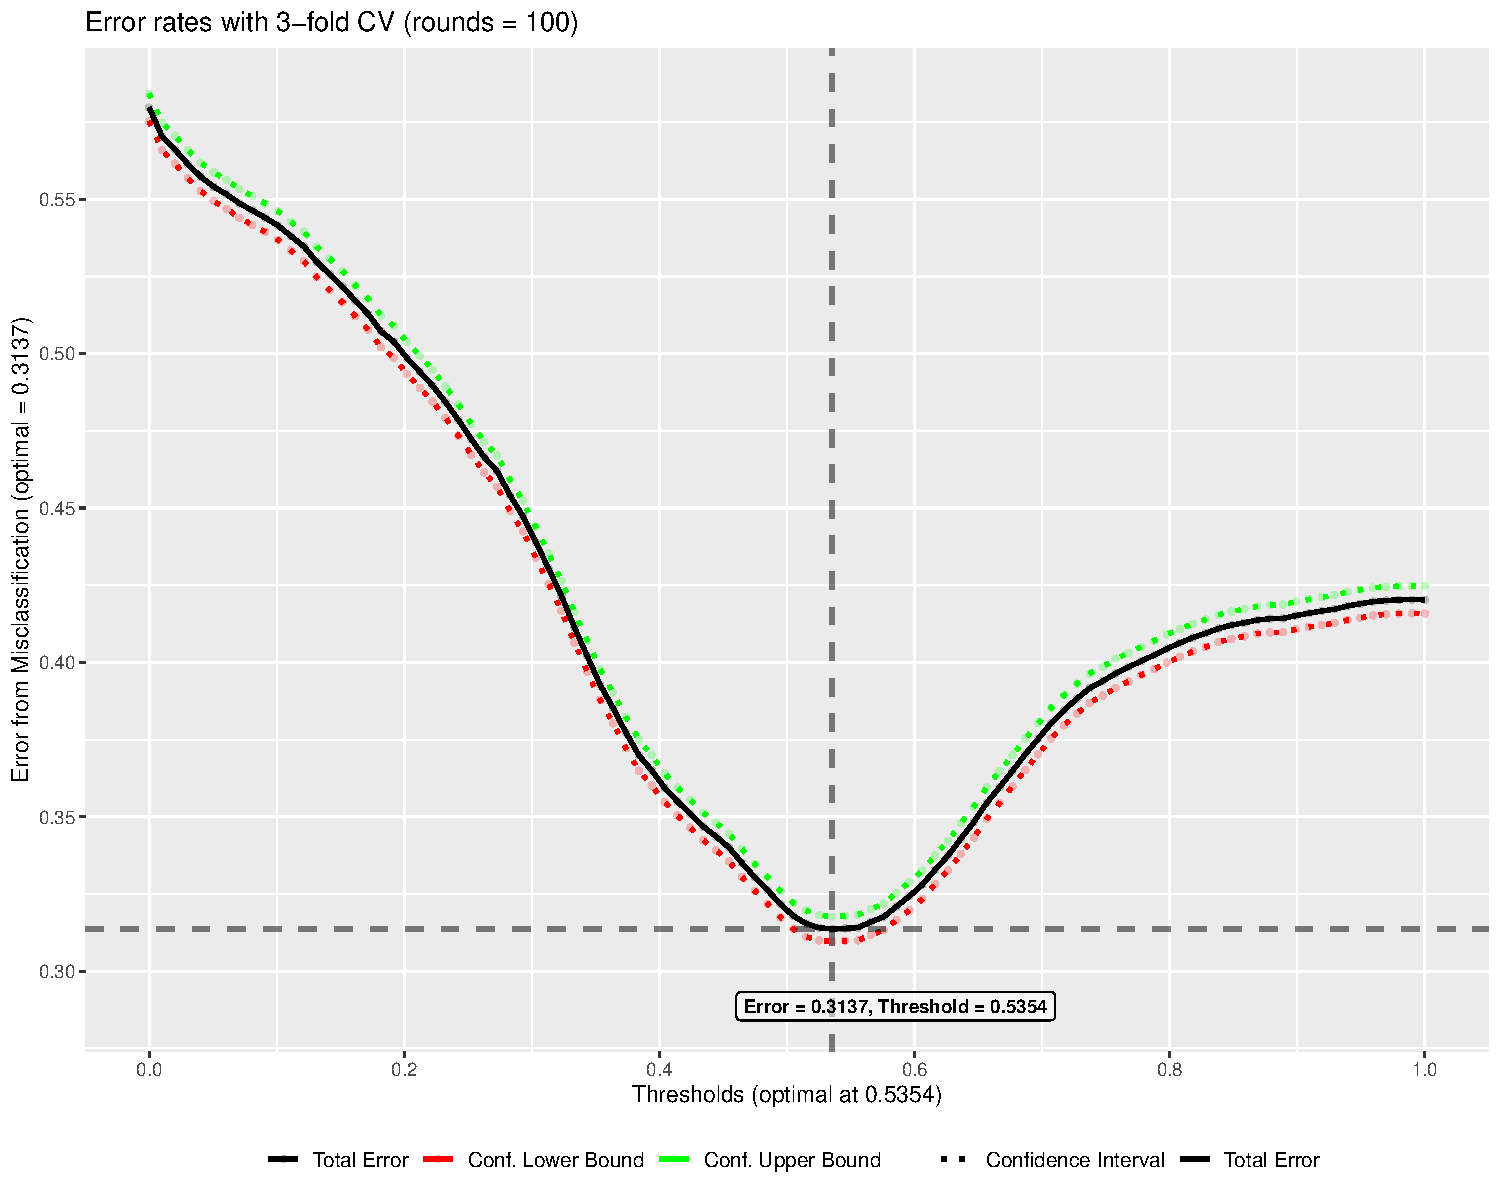
\includegraphics{figure/analysis-glm-3cv-plot-1} \end{center}

\begin{verbatim}
## $plot
## 
## $optimal_threshold
## [1] 0.5354
\end{verbatim}

\begin{verbatim}
## Optimal threshold: 0.535353535353535
## $mean
##        [,1]  [,2]
## [1,] 167.95 76.41
## [2,]  32.05 68.59
## 
## $sterr
##        [,1]   [,2]
## [1,] 0.3279 0.2899
## [2,] 0.3279 0.2899
\end{verbatim}

\newpage

\hypertarget{session-information}{%
\subsection{Session Information}\label{session-information}}

\emph{This document was generated from an
\href{http://rmarkdown.rstudio.com}{R Markdown} Notebook (See the
\texttt{vignettes/HW3\_report.Rmd} in the project's sub-directory). The
setup chunk for this document sets the root directory to the project
root directory using the \texttt{here} package; all file paths are
relative to the project root.}

\begin{verbatim}
## R version 4.1.1 (2021-08-10)
## Platform: x86_64-w64-mingw32/x64 (64-bit)
## Running under: Windows 10 x64 (build 19043)
## 
## Matrix products: default
## 
## locale:
## [1] LC_COLLATE=English_United States.1252 
## [2] LC_CTYPE=English_United States.1252   
## [3] LC_MONETARY=English_United States.1252
## [4] LC_NUMERIC=C                          
## [5] LC_TIME=English_United States.1252    
## 
## attached base packages:
## [1] stats     graphics  grDevices datasets  utils    
## [6] methods   base     
## 
## other attached packages:
##  [1] dplyr_1.0.7    tidyr_1.1.4    forcats_0.5.1 
##  [4] ggplot2_3.3.5  foreach_1.5.1  magrittr_2.0.1
##  [7] mime_0.12      markdown_1.1   rmarkdown_2.11
## [10] knitr_1.36    
## 
## loaded via a namespace (and not attached):
##  [1] highr_0.9        jquerylib_0.1.4  compiler_4.1.1  
##  [4] pillar_1.6.3     iterators_1.0.13 tools_4.1.1     
##  [7] corrplot_0.90    bit_4.0.4        digest_0.6.28   
## [10] jsonlite_1.7.2   evaluate_0.14    lifecycle_1.0.1 
## [13] tibble_3.1.5     gtable_0.3.0     pkgconfig_2.0.3 
## [16] rlang_0.4.11     cli_3.0.1        rstudioapi_0.13 
## [19] yaml_2.2.1       xfun_0.26        fastmap_1.1.0   
## [22] stringr_1.4.0    withr_2.4.2      hms_1.1.1       
## [25] generics_0.1.0   vctrs_0.3.8      bit64_4.0.5     
## [28] rprojroot_2.0.2  grid_4.1.1       tidyselect_1.1.1
## [31] glue_1.4.2       here_1.0.1       R6_2.5.1        
## [34] fansi_0.5.0      vroom_1.5.5      farver_2.1.0    
## [37] tzdb_0.1.2       readr_2.0.2      purrr_0.3.4     
## [40] scales_1.1.1     codetools_0.2-18 htmltools_0.5.2 
## [43] ellipsis_0.3.2   colorspace_2.0-2 renv_0.14.0     
## [46] utf8_1.2.2       stringi_1.7.5    munsell_0.5.0   
## [49] crayon_1.4.1
\end{verbatim}

\end{document}
